\documentclass[12pt]{article}\usepackage[]{graphicx}\usepackage[]{color}
% maxwidth is the original width if it is less than linewidth
% otherwise use linewidth (to make sure the graphics do not exceed the margin)
\makeatletter
\def\maxwidth{ %
  \ifdim\Gin@nat@width>\linewidth
    \linewidth
  \else
    \Gin@nat@width
  \fi
}
\makeatother

\definecolor{fgcolor}{rgb}{0.345, 0.345, 0.345}
\newcommand{\hlnum}[1]{\textcolor[rgb]{0.686,0.059,0.569}{#1}}%
\newcommand{\hlstr}[1]{\textcolor[rgb]{0.192,0.494,0.8}{#1}}%
\newcommand{\hlcom}[1]{\textcolor[rgb]{0.678,0.584,0.686}{\textit{#1}}}%
\newcommand{\hlopt}[1]{\textcolor[rgb]{0,0,0}{#1}}%
\newcommand{\hlstd}[1]{\textcolor[rgb]{0.345,0.345,0.345}{#1}}%
\newcommand{\hlkwa}[1]{\textcolor[rgb]{0.161,0.373,0.58}{\textbf{#1}}}%
\newcommand{\hlkwb}[1]{\textcolor[rgb]{0.69,0.353,0.396}{#1}}%
\newcommand{\hlkwc}[1]{\textcolor[rgb]{0.333,0.667,0.333}{#1}}%
\newcommand{\hlkwd}[1]{\textcolor[rgb]{0.737,0.353,0.396}{\textbf{#1}}}%
\let\hlipl\hlkwb

\usepackage{framed}
\makeatletter
\newenvironment{kframe}{%
 \def\at@end@of@kframe{}%
 \ifinner\ifhmode%
  \def\at@end@of@kframe{\end{minipage}}%
  \begin{minipage}{\columnwidth}%
 \fi\fi%
 \def\FrameCommand##1{\hskip\@totalleftmargin \hskip-\fboxsep
 \colorbox{shadecolor}{##1}\hskip-\fboxsep
     % There is no \\@totalrightmargin, so:
     \hskip-\linewidth \hskip-\@totalleftmargin \hskip\columnwidth}%
 \MakeFramed {\advance\hsize-\width
   \@totalleftmargin\z@ \linewidth\hsize
   \@setminipage}}%
 {\par\unskip\endMakeFramed%
 \at@end@of@kframe}
\makeatother

\definecolor{shadecolor}{rgb}{.97, .97, .97}
\definecolor{messagecolor}{rgb}{0, 0, 0}
\definecolor{warningcolor}{rgb}{1, 0, 1}
\definecolor{errorcolor}{rgb}{1, 0, 0}
\newenvironment{knitrout}{}{} % an empty environment to be redefined in TeX

\usepackage{alltt}
\usepackage[utf8]{inputenc} 
\usepackage{amsmath,amsfonts,amssymb,amsthm}
\usepackage[spanish, es-tabla]{babel}
\usepackage[auth-sc,affil-sl]{authblk}
%\usepackage[latin1]{inputenc}
\usepackage[spanish]{babel}
\decimalpoint
\usepackage{graphicx}
\usepackage{natbib}
\usepackage{subfig}

%\usepackage[style=authoryear]{biblatex}
\usepackage[left=2cm,right=2cm,top=2cm,bottom=2cm]{geometry}
\usepackage{setspace}
\usepackage[all]{xy}
%\usepackage{fullpage}
\usepackage{longtable}
%\usepackage {fancyvrb}
\usepackage{fancyhdr}
%\usepackage{color}
\usepackage{pstricks}
\usepackage{amsthm}
%\usepackage{harvard}
\usepackage{float}
\usepackage{footmisc}
%\usepackage[]{draftwatermark}
%\SetWatermarkText{18 de Diciembre-Versi\'on global}
%\SetWatermarkLightness{0.8}
%\SetWatermarkScale{2}

% 
\setlength{\parindent}{0pt}
\setlength{\textwidth}{6.3in}
\setlength{\topmargin}{-33pt}
\setlength{\oddsidemargin}{0pt}
\setlength{\evensidemargin}{0pt}
\setlength{\textheight}{8in}


% cosas del authblk
\setlength{\parskip}{20pt}
\setlength{\affilsep}{1mm}
\renewcommand\Authfont{\small} %\scshape\normalsize
\renewcommand\Affilfont{\itshape\small}

\renewcommand\Authsep{  }
\renewcommand\Authand{ }
\renewcommand\Authands{ }

\newcommand{\abs}[1]{ \lvert #1 \rvert }
\newcommand{\sii}{\Leftrightarrow}
\newcommand{\limi}{\liminf_n A_n}
\newcommand{\lims}{\limsup_n A_n}
\newcommand{\then}{\Rightarrow}
\newcommand{\RR}{\mathbb{R}}
\newcommand{\norm}[1]{\lvert \lvert #1 \rvert \rvert}
\newcommand{\prob}{\stackrel{p}{\to}}
\newcommand{\ton}{\stackrel{n}{\to}\,}
\newcommand{\E}{\mathbb{E} \,}
\newcommand{\limn}{\lim_{n\to +\infty}}
\newcommand{\cuadro}[3]{\setbox0\hbox{#1 \hspace{-1em}\raisebox{1em}{$\downarrow$}} \clap{\hbox to \wd0{\raisebox{#2\height}{#3}}}\box0 \;}
\newcommand{\cuadrodos}[3]{\setbox0\hbox{#1}  \llap{\hbox to \wd0{\raisebox{#2\height}{#3}}}\box0 \;}
\newcommand{\cs}{\stackrel{c.s.}{\to}}
\newcommand{\ind}[1]{1\hspace{-0.35em}1_{ \{ #1 \} } }
\newcommand{\mean}[1]{\bar{#1}_n}
\newcommand{\MAS}{$X_1, \dots, X_n$ MAS de $X$ }
\newcommand{\minim}{X_{(1:n)}}
\newcommand{\p}{\mathbb{P}}
\newcommand{\up}[1]{\stackrel{\text{#1}}{=}}
\newcommand{\f}{\mathcal{F}}
\newcommand{\bb}[1]{\bold{#1}}
\newcommand{\prodi}[1]{\left\langle #1 \right\rangle}
%\newcommand{\norm}[1]{\left\langle #1 \right\rangle}

\usepackage{tikz}
\usetikzlibrary{automata,arrows,positioning,calc}
\graphicspath{{../graf/}}


% definiciones
\newcommand{\keywordname}{Palabras clave}
\newenvironment{keywords}{%
	\paragraph*{\keywordname: }}%
{}{}
\newcommand{\area}{{\bf Área:} {\sc Métodos Matemático-Cuantitativos.}}%{\small}

%********************************************%********************************************%********************************************






\IfFileExists{upquote.sty}{\usepackage{upquote}}{}
\begin{document}
	
	\thispagestyle{empty} 
	\begin {center}
	
\includegraphics[width=0.40\textwidth]{logo_iesta.png}
		
	UNIVERSIDAD DE LA REPÚBLICA
	
	Facultad de Ciencias Económicas y Administración

	Instituto de Estadística\\
	\vspace{4.5 cm}
\textbf{\Large Titulo}	
\vspace{1.5 cm}
	
\textbf{Manuel Hernández Banadik};
\textbf{Ignacio Álvarez-Castro}\\
\vspace{0.5 cm}
	
\textbf{Abril, 2019}
\end{center}
\vspace{1.5cm}

\begin{center}
{\Huge \textbf{Serie Documentos de Trabajo}}\\
\vspace{1.0 cm}
\noindent  DT (numero) - ISSN : 1688-6453 
\end{center}
\pagebreak
\thispagestyle{empty} 
\vspace{15.5cm}

Forma de citación sugerida para este documento: 
\begin{flushleft}
\textbf{queda de postre ... }
\end{flushleft}

\newpage

\setcounter{page}{1} 
\thispagestyle{empty} 

\begin{center}
	\textbf{Titulo ... }
\end{center}

\begin{center}
  Manuel Hernández Banadik \footnote{\emph{email: }\texttt{mhernandez@iesta.edu.uy}, ORCID: 0000-0002-2505-4238\label{fn:foot_Manuel}};	Ignacio Álvarez-Castro \footnote{\emph{email: }\texttt{nachalca@iesta.edu.uy}, ORCID: 0000-0003-3123-2165\label{fn:foot_Nacho}}\\
		{\small \emph{Instituto de Estadística, Facultad de Ciencias Económicas y de Administración, Universidad de la República}}
\end{center}

\begin{center}
\textbf{RESUMEN}
\end{center}

Contamos con datos de mediciones diarias de temperaturas mínimas y máximas, de una estación meteorológica de Uruguay, desde Enero-1950 a Octubre-2014.

Se define una ola de frío, como un período de tiempo en el cual, la temperatura observada es inferior a un umbral. El objetivo es determinar dicho umbral a través de la estimación del percentil 10 de las temperaturas. Utilizaremos los modelos lineales dinámicos para modelar la serie, y para la estimación de los percentiles.

\section{Introducción}
El estudio de eventos extremos ha tomado una gran relevancia en los últimos años debido principalmente al gran impacto que presentan en la sociedad y la economía de los países, así como en los ecosistemas. Dentro de la región del Sudeste de Sudamérica los principales eventos climáticos extremos que han sido analizados son los relacionados con la temperatura (olas de calor y de frío, heladas, días cálidos, etc) y a la precipitación (sequías, precipitaciones intensas, etc). Muchos de estos estudios son relativamente actuales, debido principalmente a que es necesario contar con series temporales lo suficientemente largas y fundamentalmente completas, a un paso temporal de por lo menos un día y de alta calidad. 

Bajo el escenario de cambio climático, es necesario comprender cómo los eventos extremos cambian en frecuencia y/o intensidad, identificando cómo se han comportado en las últimas 3 o 4 décadas. Identificar este tipo de eventos ayudará a comprender su dinámica para luego realizar previsiones a un plazo menor asociado a la variabilidad climática y hasta incluso estudiar el comportamiento a escala sinóptica o de días. Uruguay cuenta con registros suficientemente largos en ciertos puntos del país, pero se han detectado muchos períodos sin información, tanto para temperaturas extremas diarias como para la variable precipitación (Renom, 2009; Amiel, 2012)

En este trabajo se presenta la estimación y caracterización de olas de frio en una estación meteorológica basadas en modelos dinámicos de la serie de temperaturas diarias máximas y mínimas en dicha estación. 

La siguiente sección presenta los datos utilizados y una definición de ola de frío. Luego, en la sección \ref{DLM} introducimos la familia de Modelos Lineales Dinámicos, que fueron usados para modelar los datos, así como la estimación de los percentiles. En la sección \ref{implementacionR} mostramos la implementación en \textbf{R} de la estimación de un modelo simulado. En la sección \ref{DLMtemp} aplicamos la metodología descripta a los datos de temperaturas de Uruguay y presentamos los resultados.

\section{Los datos}


Contamos con información de la temperatura máxima y mínima diaria en la estación meteorológica Estanzuela para el período 1951 a 2014. Definimos $\{Y^n_{t}\}$ y $\{Y^x_{t}\}$ la serie diaria de temperaturas mínima y máxima respectivamente.
%Definimos $\{Y^n_{at}\}$ y $\{Y^x_{at}\}$ la serie diaria de temperaturas mínima y máxima respectivamente, para $t \in \{1,\dots, 365\}$ y $a \in \{1950,\dots, 2014\}$ (\textcolor{blue}{te parece bien esta notación?? si es asi hay que adaptar todo lo demás a esto})

Existen diversas formas de caracterizar una racha de frío, que responden a distintas aplicaciones de su estudio. Las diversas definiciones acuerdan en la necesidad de establecer un umbral de bajas temperaturas (puede ser absoluto o relativo) y en delimitar una ventana de tiempo durante la cual, la temperatura observada debe mantenerse por debajo del umbral definido. 

En el presente trabajo, hemos definido una ola de frío como un período de tiempo mayor o igual a 3 días, en los cuales las temperaturas mínimas y máximas son inferiores a los respectivos percentiles 10 esperados para tales días. Definimos el percentil 10 de mínima como $p^n_{10_t}:= \inf\{y: \p(Y^n_t \leq y)\geq 0.1\}$. Análogamente definimos el percentil 10 de máxima para el día $t$ como $p^x_{10_t}:= \inf\{y: \p(Y^x_t \leq y)\geq 0.1\}$. Podemos decir entonces que una sucesión de días $t_1, \dots, t_k$ constituyen una ola de frío de largo $k$ si, siendo $k\geq 3$, se cumple simultáneamente que:

$\begin{cases} y^n_{t_i} < p^n_{10_i}  \\ y^x_{t_i} < p^x_{10_i} \end{cases}$ para $i=1,\dots,k$

Vizualizar fenómenos de olas de extremos no es trivial, aplicando la definición anterior, debemos tenr en cuenta varios factores. En primer lugar la condición recae simultaneamente sobre la temperatura mínima y máxima por lo que debemos prestar atención a ambas series. Al mismo tiempo debemos comparar la temperatura de cada día en particular con los percentiles para ese día, o más en general, con las temperaturas esperables. Finalmente, los días deben ser consecutivos para formar una ola de extremos. 

La figura \ref{fig:graf1} muestra las series de temperaturas para el año 2012 (\textcolor{blue}{la serie es del 2012 o 2011 ???}) su la distribución de frecuencias. El gráfico tiene 3 capaz básicas, en primer lugar calculamos un histograma bidimensional en que los bins son hexágonos en el plano de $\{ y^n_{ta}, t$ (panel superior), la intensidad del color representa la frecuencia. Sobre el histograma se dibuja las series de temperatura observada para cada día en 2012 y finalmente se divide en dos paneles con la serie de mínima (superior) y máxima (inferior) por separado. 

\begin{knitrout}
\definecolor{shadecolor}{rgb}{0.969, 0.969, 0.969}\color{fgcolor}\begin{figure}

{\centering 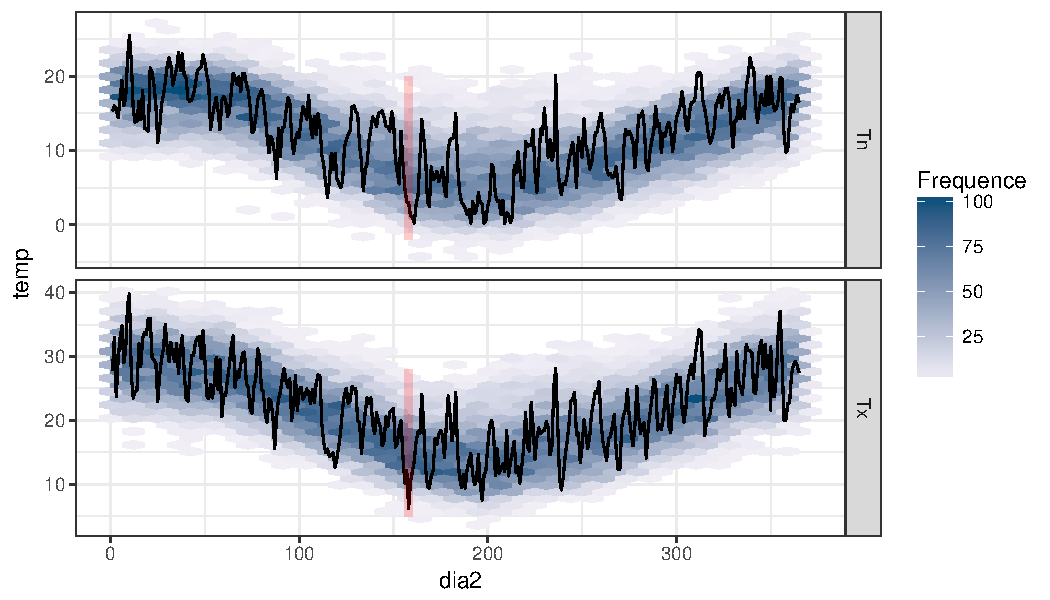
\includegraphics[width=\maxwidth]{figure/graf1-1} 

}

\caption[Gráfico]{Gráfico}\label{fig:graf1}
\end{figure}


\end{knitrout}
\textcolor{blue}{en la figura: caption con descripcion, nombres de los ejes y la etiqueta de color, nombres de los paneles}

El período de días del 5 al 9 de junio de 2012 (señalado en rojo en la Figura \ref{fig:graf1}) la temperatura observada se acerca a la cola inferior de la distribución para ese día. Eso indica que ese período fue bastante más frio de lo esperado, podemos considerar que durante esos días estuvimos ante la presencia de una \textit{ola de frío}. 

\textcolor{blue}{comentario de cierre??}

\section{Modelos lineales dinámicos}\label{DLM}

%Los modelos lineales dinámicos (DLM) son una familia de modelos de espacio de estado. Procesos muy conocidos pueden ser vistos como modelos DLM: el paseo al azar, el modelo de regresión normal, los modelos ARIMA, entre otros.
%
%Un modelo estadístico de posición, establece que hay un parámetro del cual tenemos observaciones ruidosas. %Podemos extender esa idea, y considerar que tenemos obervaciones ruidosas de un
%Podemos extender la idea de parámetro 

Los modelos lineales dinámicos (DLM) son una familia de modelos que constituye una subclase de los llamados modelos de espacio de estado. En DLM se considera una serie de tiempo, $Y_t$, como una observación ruidosa de un proceso dinámico no observable $\theta_t$. Estos modelos se definen a través de dos ecuaciones básicas: una \textit{ecuación de evolución} y una \textit{ecuación de observación}. La estructura general de un DLM se muestra en \eqref{ecu.obs} y \eqref{ecu.evo} donde $F_t$ $G_t$ son dos matrices conocidas de orden $p\times p$ y $m\times p$ respectivamente que caracterizan al modelo, las perturbaciones $v_t$ y $w_t$ son son secuencias de vectores gausianos independientes, mientras que $V_t,W_t$ serán los parámetros que caractericen el modelo. Adicionalmete, se agrega una previa Normal para el momento inicial, es decir $\theta_0 \sim N(m_0, C_0)$. 

\begin{eqnarray}
\label{ecu.obs} Y_t&= F_t\theta_t + v_t  \;&\;  v_t \sim \mathcal{N}(0,V_t) \\
\label{ecu.evo} \theta_t &= G_t \theta_{t-1} + w_t \;&\; w_t \sim \mathcal{N}(0,W_t)
%\label{eq:modelo}
\end{eqnarray} 

La ecuación de evolución responde a la dinámica del proceso estocástico: define cómo se vincula el estado del proceso en tiempo $t$ con su estado en tiempo $t+1$. Por otro lado, la ecuación de observación, explicita cómo es observado el proceso en tiempo $t$ dado el estado en el que se encuentra a tiempo $t$. En ambas ecuaciones, se puede introducir una componente aleatorio. 

\subsection{Estructura de un DLM}

La estructura de depencia entre las observaciones es un aspecto clave para entender como funcionan los DLM. Al igual que la clase maás general de modelos espacio-estado en los DLM se basa en dos supuestos fundamentales. En primer lugar se asume  que el proceso inobservable o proceso de estado $\theta_t$ consituye una cadena de Markov.  En tanto, las observaciones $Y_t$ son condicionalmente independientes dado $\theta_t$ y se asume que $Y_t$ depende únicamente de $\theta_t$. 

\begin{center}
\begin{tikzpicture}[->, >=stealth', auto, semithick, node distance=3cm]
\tikzstyle{every state}=[fill=white,draw=black,thick,text=black,scale=1]
\node[state]    (A)                     {$\theta_t$};
\node[state]    (B)[above of=A]   {$Y_t$};
\node[state]    (D)[right of=A]   {$\theta_{t+1}$};
\node[state]    (C)[above of=D]   {$Y_{t+1}$};
\node[state]    (E)[left of=A]   {$\theta_{t-1}$};
\node[state]    (F)[left of=B]   {$Y_{t-1}$};
\path
(E) edge[right]     node{}         (A)
(A) edge[left]     node[label={[shift={(0.15,-.6)}] \scriptsize{evolución}}] {}         (D)
%     edge[bend left]     node{$(1-p)^2$}     (B)
%     edge[bend left,below]      node{$p(1-p)$}      (D)
%     edge[bend right]    node{$p(1-p)$}      (C)
% (B) edge                node{$1$}           (D)
% (C) edge                node{$1$}           (D)
% (D) edge[loop right]    node{$(1-q)^2$}     (D)
%     edge[bend right,right]    node{$q(1-q)$}      (B)
%     edge[bend left]     node{$q(1-q)$}      (C)
(E)    edge (F)
(D) edge (C)
(A)    edge[above]     node[label={[shift={(0.85,-0.5)}] \scriptsize{observación}}] {}         (B);

%\node[above=0.5cm] (A){Patch G};
%\draw[red] ($(D)+(-1.5,0)$) ellipse (2cm and 3.5cm)node[yshift=3cm]{Patch H};
\end{tikzpicture}
\captionof{figure}{Diagrama de evolución y observación del proceso}\label{diagrama}
\end{center}

La figura \ref{diagrama} representa un diagrama de la estructura de depndencia en DLM, donde los arcos indican dependencia estadistica. Se puede ver como  $\theta_t$, toda la dependencia entre observaciones pasa a través del proceso latente. A partir de esta estructura, se puede considerar que las observaciones representan una medida ruidosa el proceso de estado.

La principal consecuencia de la estructura de dependencia es que la distribucion conjunta de todas las variables de interes queda determinada por la distribucion previa del estado inicial y las densidades condicionales $p(\theta_t | \theta_{t-1})$, $p(y_t|\theta_t)$, de forma: 
\[
p(\theta_{0:t}, y_{1:t}) =  p(\theta_0) \prod_{j=1}^t  p(\theta_j | \theta_{j-1})  p(y_j|\theta_j)
\]

La famillia de DLM es amplia y flexible, muchos modelos estadisticos para datos temporales pueden verse como casos partiulares de esta familia o de la clase mas general de modelos espacio-estados. En particular los modelos ARMA con ruido gaussiano son equivalentes a DLM cuando los parametros $F_t, G_t, V_t, W_t$ son constantes en el tiempo. Por ejemplo, el proceso  AR(2): $y_t = \phi_1 y_{t-1} + \phi_2 y_{t-2} + e_t$, puede ser visto como un DLM si definimos $\theta_t = 
\begin{pmatrix}
\theta_{1,t} \\
\theta_{2,t}
\end{pmatrix}
$
y luego, 

\[ \begin{array}{rl}
y_t = & \begin{bmatrix}
1 \\
0
\end{bmatrix}
\theta_t = \theta_{1,t} \\
& \\
\theta_t = \begin{pmatrix} \theta_{1,t} \\ \theta_{2,t} \end{pmatrix} = &
\begin{bmatrix} \phi_1 & 1 \\ \phi_2 & 0 \end{bmatrix}
\begin{pmatrix} \theta_{1,t-1} \\ \theta_{2,t-1} \end{pmatrix}
+
\begin{bmatrix} e_t \\ 0 \end{bmatrix}
\end{array}
\]
para ver la equivalencia entre ambas representaciones, debemos operar en la segunda ecuación, que representa la evolución del proceso latente y verificar que se verifica que $\theta_{1,t} = \phi_1 \theta_{1,t-1} + \phi_2 \theta_{1,t-2} + e_t$. Ver CITA.LIBRO (sección 3.2.5) por más detalles en la correspondencia entre modelos ARIMA($p$, $d$, $q$) y DLM. 

Aparte de DLM, la familia de modelos espacio-estados admite modelos no lineales y el uso de otras distribuciones no Gausianas. Por ejemplo, modelos para las distribuciones de la familia exponencial pueden ser especificados para tener DLMG \textit{generalizados}, por otro lado en casos uqe el proceso de estados tenga una distribucion discreta el modelo es referido como modelos ocultos de MArkov, tambien modelos de volatilidad estocastica pueden ser vistos como espacio-estados. El estudio de DLM entonces, es relevante pues permite introucirnos al trabajo con una familia de modelos que es muy amplica y puede aplicarse en una gran variedad de problemas concretos. 


\begin{center}
$\begin{array}{lc}
Y_t=F_t\theta_t + v_t  &  v_t \sim \mathcal{N}(0,V_t) \\
\theta_t = G_t \theta_{t-1} + w_t \;\; & w_t \sim \mathcal{N}(0,W_t)
\end{array}$
\end{center}

\subsection{Estimacion del proceso de estados}

Si se tienen las observaciones $y_1,\dots,y_T$, y se asume un modelo como el descripto por las ecuaciones \eqref{ecu.obs} y \eqref{ecu.evo}, hay varias distribuciones posteriores que puede ser de interes. En relacion al proceso no observable se distinguen tres distribuciones relevantes condicional en los datos observados: filtrada, suavisada y de prediccion.

La \textbf{distribucion filtrada} (filtering distribution en ingles) consiste en la distribucion del estado no observable $\theta_t$ dada la informacion observada hasta ese mismo momento, es decir $p(\theta_t | y_{1:t}$, se tiene una distribucion para cada momento $t$. La posterior filtrada es de principal interes en aplicaciones secuenciales donde es necesario realizar una nueva estimacion para cada observacion nueva. 

En el caso de modelos DLM descritos por \eqref{ecu.obs} y \eqref{ecu.evo}, donde operan las restricciones de normalidad y linealidad, es posible tener soluciones cerradas para $p(\theta_t | y_1, \ldots, y_t)$ mediante el Filtro de Kalman. El filtro de Kalman puede verse como la resolucion recursiva de un problema de estimacion Bayesiana en el modelo lineal gaussiano, distribucion posterior de interes es $p(\theta_t | y_{1:t} )$, que se obtiene como
\[
p(\theta_t | y_{1:t}) = \frac{ p(y_t | \theta_t) p(\theta_{t} | y_{1:t-1})}{ p(y_t | y_{1:t}  }
\]
En primer lugar, suponemos conocida la distribucion filtrada del paso anterior, $p(\theta_{t-1} | y_{1:t-1}) = N(m_{t-1}, C_{t-1})$. Luego, como la ecuacion \eqref{ecu.evo} implica que $ p(\theta_{t} | \theta_{t-1} = N(G_t\theta_{t-1}, W_t)$ se puede obtener la distribucion previa $p(\theta_{t} | y_{1:t-1}$ como en \eqref{ecu.previa}. Es simple mostrar que el resultado es que la previa para el estado $\theta_t$ es normal, $\theta_t |y_{1:t-1} \sim N(a_t, R_t)$, donde $a_t = G_tm_{t-1}$ y $R_t = G_t C_{t-1} G_t^{\top} + W_t$. 
\begin{equation}
p(\theta_{t} | y_{1:t-1})  \int  p(\theta_{t} | \theta_{t-1}) p( \theta_{t-1}|y_{1:t-1}) d\theta_{t-1} \\
\label{ecu.previa}
\end{equation}

Por otro lado, la verosimilitud $p(y_t | \theta_t)$ es tambien normal, esto surge directamente de \eqref{ecu.obs} en que se explicita que $y_t | \theta_t \sim N(F_t \theta_t, V_t)$. Con estos ingredientes, modelo de datos y previa gaussianas, podemos obtener la posterior de interees aplicadndo resultados conocidos de modelo de regresion lineal conjugado para obtener el resultado del filtro de Kalman como 
\[\begin{array}{ccc}
\theta_t | y_{1:t} \sim N(m_t, C_t) & m_t = C_t( R_t^{-1}a_t + F_t^{\top}V_t^{-1}y_t ) & C_t = (R_t^{-1} + F_t^{\top}V_t^{-1}F_t)^{-1}
\end{array}
\]
Utilizando la previa normal para el momento inicial ($\theta_0$) se procede iterativamente para obtener la distribucion filtrada para todos los estados latentes $\theta_1$ a $\theta_T$. 

Una segunda distribucion posterior que puede tener relevancia en aplicaciones es la \textbf{distribucion suavizada} (smoothing distribution en ingles) del proceso de estados. La distribucion suavizada consiste en $p(\theta_t | y_1, \ldots, y_T)$, es similar a la posterior filtrada con la diferencia que el condicional se realiza sobre todos los datos observados disponibles. La distribucion suavizada es relevante para aplicaciones donde estamos interesados en un estudio retrospectivo y se desea analizar todo el proceso de estados latente. \textcolor{blue}{a nosotros no deberia interesarnos mas smoothing que filtering ???}

\textcolor{blue}{estimacion de los parametros de varianza? MLE.. otra forma?}

En caso que estemos interesados en predecir un valor futuro del estado se utilizan distribuciones de prediccion $p(\theta_{t+k} | y_1, \ldots, y_t)$. \textcolor{blue}{expandir y comentar sobre predictiva de observaciones}

\textcolor{blue}{Incluir tratamiento de datos faltantes, caapz que para que se entienda son necesarias incluir formulas para calcular filtering y smoothing}

 
\subsection{Un ejemplo simulado \label{implementacionR} }
%\subsection{Implementación computacional en \textbf{R}}\label{implementacionR}
En lo que sigue se ilustra la estimación de DLM mediante un ejemplo simulado de un proceso simple y su estimación mediante la biblioteca \verb|dlm| (CITA??) que permite trabajar con toda la familia de modelos lineales dinámicos. La ecuación \eqref{dlm_sim} muestra el modelo usado para simular datos,  en este caso $G_t$ y $F_t$ se definieron constantes con valor 1. El proceso de estado $\{\theta_t\}$ describe un paseo al azar, mientras que podemos considerar a $\{y_t\}$ como una observación ruidosa de $\{\theta_t\}$. El objetivo será recumerar los valores de los parámetros de varianzas y el proceso de estado. \textcolor{blue}{notar que no es estacionario...}

\begin{equation}
\begin{aligned}
Y_t&=\theta_t + v_t  \;&\;  v_t \sim \mathcal{N}(0,0.1^2) \\
\theta_t &= \theta_{t-1} + w_t \;&\; w_t \sim \mathcal{N}(0,0.3^2)
\end{aligned}
\label{dlm_sim}
\end{equation}
 
El siguiente código de  \textbf{R} realiza la simulación de un conjunto de datos con el modelo descrito en \eqref{dlm_sim} y su estimación con el Filtro del Kalman.
\begin{knitrout}
\definecolor{shadecolor}{rgb}{0.969, 0.969, 0.969}\color{fgcolor}\begin{kframe}
\begin{alltt}
\hlcom{# Obtenemos estados y datos simulados}
\hlkwd{set.seed}\hlstd{(}\hlnum{1237}\hlstd{); N} \hlkwb{<-} \hlnum{100}

\hlstd{dd} \hlkwb{<-} \hlkwd{data_frame}\hlstd{(}\hlkwc{t} \hlstd{=} \hlkwd{seq}\hlstd{(}\hlnum{0}\hlstd{,}\hlnum{1}\hlstd{,} \hlkwc{length.out} \hlstd{= N),} \hlkwc{w} \hlstd{=} \hlkwd{rnorm}\hlstd{(N,}\hlnum{0}\hlstd{,}\hlnum{.1}\hlstd{),} \hlkwc{v} \hlstd{=} \hlkwd{rnorm}\hlstd{(N,}\hlnum{0}\hlstd{,}\hlnum{.3}\hlstd{) )} \hlopt
  \hlkwd{mutate}\hlstd{(} \hlkwc{theta} \hlstd{=} \hlkwd{cumsum}\hlstd{(w),} \hlkwc{y} \hlstd{=} \hlkwd{ts}\hlstd{(theta} \hlopt{+} \hlstd{v) )}

\hlcom{# Función para estimar varianzas por Max.Ver}
\hlstd{parMLE} \hlkwb{<-} \hlkwa{function}\hlstd{(}\hlkwc{par}\hlstd{)} \hlkwd{dlmModPoly}\hlstd{(}\hlnum{1}\hlstd{,} \hlkwc{dV} \hlstd{= par[}\hlnum{1}\hlstd{],} \hlkwc{dW} \hlstd{= par[}\hlnum{2}\hlstd{])}
\hlstd{modPoly} \hlkwb{<-} \hlkwd{dlmMLE}\hlstd{(dd}\hlopt{$}\hlstd{y,}\hlkwc{parm} \hlstd{=} \hlkwd{c}\hlstd{(}\hlnum{1}\hlstd{,}\hlnum{1}\hlstd{),}\hlkwc{build} \hlstd{= parMLE)}

\hlcom{# Kalman filter y Kalman smoother}
\hlstd{mod_filter} \hlkwb{<-} \hlkwd{dlmFilter}\hlstd{(dd}\hlopt{$}\hlstd{y,} \hlkwd{parMLE}\hlstd{(modPoly}\hlopt{$}\hlstd{par))}
\hlstd{mod_smooth} \hlkwb{<-} \hlkwd{dlmSmooth}\hlstd{(mod_filter)}
\end{alltt}
\end{kframe}
\end{knitrout}

En primer lugar, es estimar los parámetros desconocidos del modelo con la función \verb|dlmMLE()|, que aproximará una estimación óptima, con un algoritmo iterativo. Para ello, primero debemos crear una función auxiliar (\verb|parMLE()|), cuyo argumento sea un vector de valores iniciales propuesto para los parámetros que se desea estimar, en nuestro caso desconocemos $V_t$ y $W_t$, la varianza del ruido de evolución y la varianza del ruido de observación. El objeto \verb|modPoly| contiene el modelo con los parámetros estimados.

Una vez estimado el modelo, podemos aplicar el filtro de Kalman mediante (\verb|dlmFilter()|) para obtener estimaciones de la esperanza posterior,
\begin{knitrout}
\definecolor{shadecolor}{rgb}{0.969, 0.969, 0.969}\color{fgcolor}\begin{kframe}
\begin{verbatim}
## List of 9
##  $ y  : Time-Series [1:100] from 1 to 100: -0.18756 -0.226 0.05441 -0.00719 -0.21121 ...
##  $ mod:List of 10
##   ..- attr(*, "class")= chr "dlm"
##  $ m  : Time-Series [1:101] from 0 to 100: 0 -0.1876 -0.2081 -0.102 -0.0685 ...
##  $ U.C:List of 101
##  $ D.C: num [1:101, 1] 3162.278 0.289 0.211 0.184 0.172 ...
##  $ a  : Time-Series [1:100] from 1 to 100: 0 -0.1876 -0.2081 -0.102 -0.0685 ...
##  $ U.R:List of 100
##  $ D.R: num [1:100, 1] 3162.278 0.309 0.238 0.214 0.204 ...
##  $ f  : Time-Series [1:100] from 1 to 100: 0 -0.1876 -0.2081 -0.102 -0.0685 ...
##  - attr(*, "class")= chr "dlmFiltered"
\end{verbatim}
\end{kframe}
\end{knitrout}
las series de tiempo \verb|m|, \verb|a| y \verb|f| contienen la estimación del estado, la predicción del estado a un paso y la predicción de las observaciones a un paso, respectivamente. Adicionalmente, la función \verb|dlmSmooth()| aplica el suavizado de Kalman y nos devuelve la estimación suavizada del proceso de estados.

La figura \ref{fig:graf7b} muestra los resultados de la estimación modelo, en cada panel se muestran los datos observados (serie gris), el verdadero valor del estado $\theta_t$ (serie negra) y una una estimación del modelo (serie roja). Los tres tipos de estimación comentados previamente corresponden a cada panel de la figura, en el panel superior se muestra la estimación filtrada que utiliza datos hasta el momento en que se quiere estimar, es decir $m_t = E(\theta_t | y_1,\ldots, y_t)$. El panel intermedio muestra la predicción a un paso del proceso de observación, $f_t = E(y_t | y_1, \ldots, y_{t-1})$, y finalmente, el en el panel inferior se muestra la esitmación suavizada del estados, utilizando toda la información disponible para obtenerla, es decir $s_t = E(\theta_t | y_1, \ldots, y_N)$

\begin{knitrout}
\definecolor{shadecolor}{rgb}{0.969, 0.969, 0.969}\color{fgcolor}\begin{figure}

{\centering 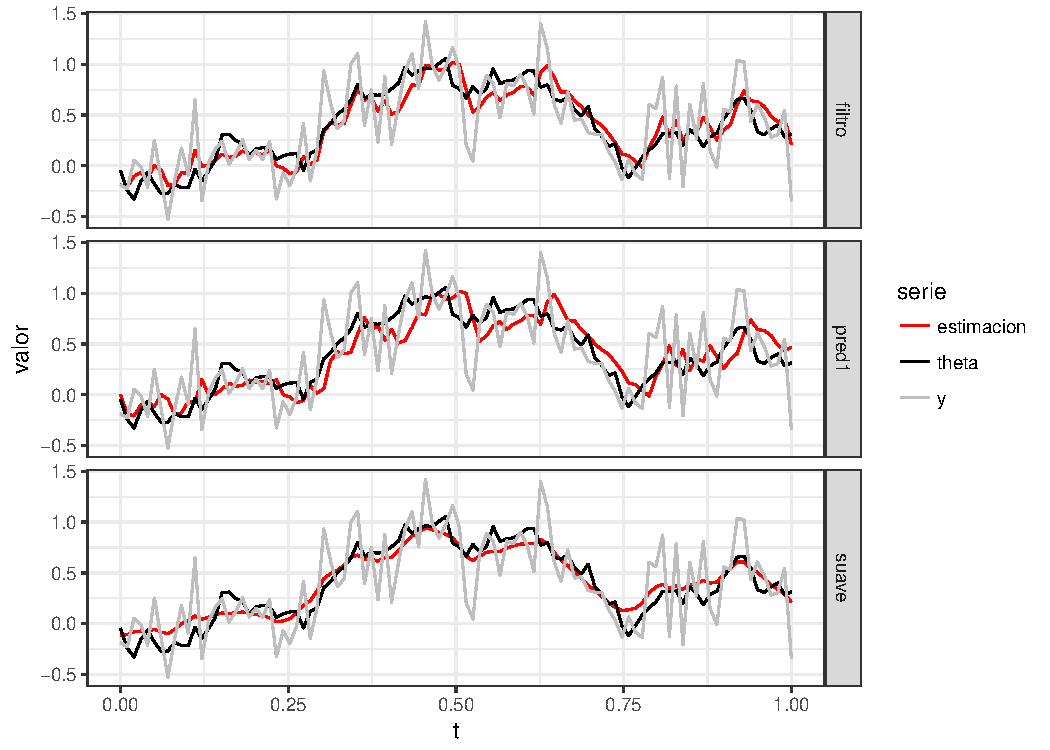
\includegraphics[width=\maxwidth]{figure/graf7b-1} 

}

\caption[Ejemplo de un proceso de espacio de estado y su estimación]{Ejemplo de un proceso de espacio de estado y su estimación.}\label{fig:graf7b}
\end{figure}


\end{knitrout}
las series de tiempo \verb|m|, \verb|a| y \verb|f| contienen la estimación del estado, la predicción del estado a un paso y la predicción de las observaciones a un paso, respectivamente. Adicionalmente, la función \verb|dlmSmooth()| aplica el suavizado de Kalman y nos devuelve la estimación suavizada del proceso de estados.

La figura \ref{fig:graf7b} muestra los resultados de la estimación modelo, en cada panel se muestran los datos observados (serie gris), el verdadero valor del estado $\theta_t$ (serie negra) y una una estimación del modelo (serie roja). Los tres tipos de estimación comentados previamente corresponden a cada panel de la figura, en el panel superior se muestra la estimación filtrada que utiliza datos hasta el momento en que se quiere estimar, es decir $m_t = E(\theta_t | y_1,\ldots, y_t)$. El panel intermedio muestra la predicción a un paso del proceso de observación, $f_t = E(y_t | y_1, \ldots, y_{t-1})$, y finalmente, el en el panel inferior se muestra la esitmación suavizada del estados, utilizando toda la información disponible para obtenerla, es decir $s_t = E(\theta_t | y_1, \ldots, y_N)$

\begin{knitrout}
\definecolor{shadecolor}{rgb}{0.969, 0.969, 0.969}\color{fgcolor}\begin{figure}

{\centering \includegraphics[width=\maxwidth]{figure/graf7c-1} 

}

\caption[Ejemplo de un proceso de espacio de estado y su estimación]{Ejemplo de un proceso de espacio de estado y su estimación.}\label{fig:graf7c}
\end{figure}


\end{knitrout}



\definecolor{theta}{HTML}{F8766F}
\definecolor{ye}{HTML}{7CAE00}
\newcommand{\thetaline}{\raisebox{2pt}{\tikz{\draw[-,theta,-,line width = 0.9pt](0,0) -- (5mm,0); }}\;}
\newcommand{\yeline}{\raisebox{2pt}{\tikz{\draw[-,ye,-,line width = 0.9pt](0,0) -- (5mm,0); }}\;}


% \vspace{-.75em}
% \captionof{figure}[Ejemplo de un proceso de espacio de estado]{Ejemplo de un proceso de espacio de estado y su estimación. %En \thetaline se representa el proceso \textit{no-observable}, en \yeline se representa su observación.
% }
% \label{fig:graf7}



\section{Modelo estacional para el modelado de temperaturas}\label{DLMtemp}
\textcolor{blue}{describir mas explicitamente el modelo utilizado, o sea, agregar la ecuacion de observacion, y comentar el porque y las consecuencias de usar W=0}

Modelaremos la serie de mínimas y máximas de forma independiente, utilizaremos el mismo modelo para ambas.

Dada la fuerte característica estacional de los datos de temperaturas, es apropiado modelarla como una función periódica más un ruido aleatorio. En este caso, el proceso latente será modelado como una función de período 365s y su dinámica no será aleatoria, esto se traduce en imponer matrices de varianza nulas para la ecuación de evolución.
Tal función está caracterizada por un vector $\alpha \in \RR^{365}$. La representación de $\alpha$ en la base canónica nos habla de su naturaleza temporal -\textit{qué temperatura esperamos cada día del año}-. Por distintos motivos será de mayor interés considerar la representación de $\alpha$ en una base de Fourier. Esto nos permitirá trabajar en un espacio de dimensión significativamente menor, con muy poca pérdida de información, dado que unos pocos armónicos (en nuestro caso 2) tienen coeficientes de fourier `significativos', definiendo así un criterio para descartar armónicos de mayor frecuencia, responsables de la rugosidad de la serie.

En este caso el modelo será:
$$\theta_t=\left(\begin{array}{lr}
S_1:=& a_1\cos\left(\frac{2\pi t}{365}\right) + b_1 \sin\left(\frac{2\pi t}{365}\right) \\
S_1^*:=& -a_1\sin\left(\frac{2\pi t}{365}\right) + b_1 \cos\left(\frac{2\pi t}{365}\right) \\
S_2:= &a_2\cos\left(\frac{4\pi t}{365}\right) + b_2 \sin\left(\frac{4\pi t}{365}\right) \\
S_2^*:=& -a_2\sin\left(\frac{4\pi t}{365}\right) + b_2 \cos\left(\frac{4\pi t}{365}\right) \\
\end{array}\right)\; F_t=(1,0,1,0) \; \forall \, t$$

La matriz $G_t$ (constante en $t$) será una matriz diagonal por bloques, cuyos dos bloques serán matrices de rotación de ángulos horarios $\frac{2\pi}{365}$ y $\frac{4\pi}{365}$. La matriz $W_t$ se definió nula. La varianza observacional $V_t$ será estimada por máxima verosimilitud.

\subsection{Estimación de percentiles}
\textcolor{blue}{modificar esto para usar kalman smoother}

Como se explicó anteriormente, para caracterizar olas de frío debemos estimar los percentiles 10 de temperaturas mínimas y máximas para cada día del año. Tenemos las series temporales de los datos de mínima y máxima, a escala diaria, desde el 1-Enero de 1950 hasta el 10-Octubre de 2014, por tanto para cada día del año (del 1-Enero al 31-Diciembre) tenemos más de sesenta observaciones de temperaturas. Esto da para cada día del año una distribución de temperaturas.  %Un acercamiento a este problema se puede ver en {\color{red}[referencia a Santiago]} donde se computa el percentil empírico para cada día del año y luego, a la serie de percentiles, se le aplica un filtro de medias móviles con una ventana de 31 días para obtener una estimación suave.

En este trabajo, para la estimación de tales percentiles, nos valdremos de la distribución de $\theta_t | \{y_1,\dots,y_t\}$. Se puede probar que, bajo el modelo descripto en la expresión (\ref{eq:modelo}), se cumple que $\theta_t | \{y_1,\dots,y_t\} \sim \mathcal{N}(m_t,C_t)$, y $y_t|\theta_t \sim \mathcal{N}(Fm_t,FC_tF^T + \text{v}_t)$. El filtro de Kalman nos devuelve las secuencias $(m_t)_{1\leq t \leq T}$ y $(C_t)_{1\leq t \leq T}$ para la serie de temperaturas mínimas y máximas. Por tanto, el estimador para el percentil 10 de mínima para el día $t$ será $\hat{p}^n_{10_t}:=Fm_t+\sqrt{FC_tF^T + \text{v}_t}\times \Phi(0.10)$, donde $\Phi(x)=\p(X\leq x)$ con $X\sim N(0,1)$. Análogamente se hace lo mismo para el percentil 10 de temperaturas máximas.

%\section{Implementación en R - paquete `dlm'}
\section{Resultados}
\textcolor{blue}{por ahora aca hay dibujos para mostrarle a Santiago...}

% El paquete \verb|dlm| permite trabajar con toda la familia de modelos lineales dinámicos. %La función \verb|dlmMoTrig| nos permite crear objetos \verb|dlm| de

Si el objeto \verb|y| contiene una de las series de temperaturas, el siguiente programa nos dará la estimación del modelo.

\begin{knitrout}
\definecolor{shadecolor}{rgb}{0.969, 0.969, 0.969}\color{fgcolor}\begin{kframe}
\begin{alltt}
\hlstd{parMLE} \hlkwb{<-} \hlkwa{function}\hlstd{(}\hlkwc{par}\hlstd{)}  \hlkwd{dlmModTrig}\hlstd{(}\hlkwc{s} \hlstd{=} \hlnum{365}\hlstd{,}\hlkwc{q}\hlstd{=}\hlnum{2}\hlstd{,} \hlkwc{dV} \hlstd{=} \hlkwd{exp}\hlstd{(par),} \hlkwc{dW} \hlstd{=} \hlnum{0}\hlstd{)}

\hlcom{# Estima el modelo para temp Minimas}
\hlstd{mod.tn} \hlkwb{<-} \hlkwd{filter}\hlstd{(d2, serie} \hlopt{==} \hlstr{'Tn'}\hlstd{)} \hlopt
  \hlkwd{mutate}\hlstd{(}\hlkwc{temp} \hlstd{= temp}\hlopt{-}\hlkwd{mean}\hlstd{(temp,} \hlkwc{na.rm} \hlstd{= T))} \hlopt \hlkwd{pull}\hlstd{(temp)} \hlopt
  \hlkwd{ts}\hlstd{(}\hlkwc{start} \hlstd{=} \hlkwd{c}\hlstd{(}\hlnum{1950}\hlstd{,} \hlnum{1}\hlstd{),} \hlkwc{frequency} \hlstd{=} \hlnum{365}\hlstd{)} \hlopt
  \hlkwd{dlmMLE}\hlstd{(} \hlkwc{parm} \hlstd{=} \hlnum{0}\hlstd{,} \hlkwc{build}\hlstd{= parMLE)}

\hlcom{# Estima el modelo para temp Maximas}
\hlstd{mod.tx} \hlkwb{<-} \hlkwd{filter}\hlstd{(d2, serie} \hlopt{==} \hlstr{'Tx'}\hlstd{)} \hlopt
  \hlkwd{mutate}\hlstd{(}\hlkwc{temp} \hlstd{= temp}\hlopt{-}\hlkwd{mean}\hlstd{(temp,} \hlkwc{na.rm} \hlstd{= T))} \hlopt
  \hlkwd{pull}\hlstd{(temp)} \hlopt
  \hlkwd{ts}\hlstd{(}\hlkwc{start} \hlstd{=} \hlkwd{c}\hlstd{(}\hlnum{1950}\hlstd{,} \hlnum{1}\hlstd{),} \hlkwc{frequency} \hlstd{=} \hlnum{365}\hlstd{)} \hlopt
  \hlkwd{dlmMLE}\hlstd{(} \hlkwc{parm} \hlstd{=} \hlnum{0}\hlstd{,} \hlkwc{build}\hlstd{= parMLE)}
\end{alltt}
\end{kframe}
\end{knitrout}



\begin{knitrout}
\definecolor{shadecolor}{rgb}{0.969, 0.969, 0.969}\color{fgcolor}

{\centering 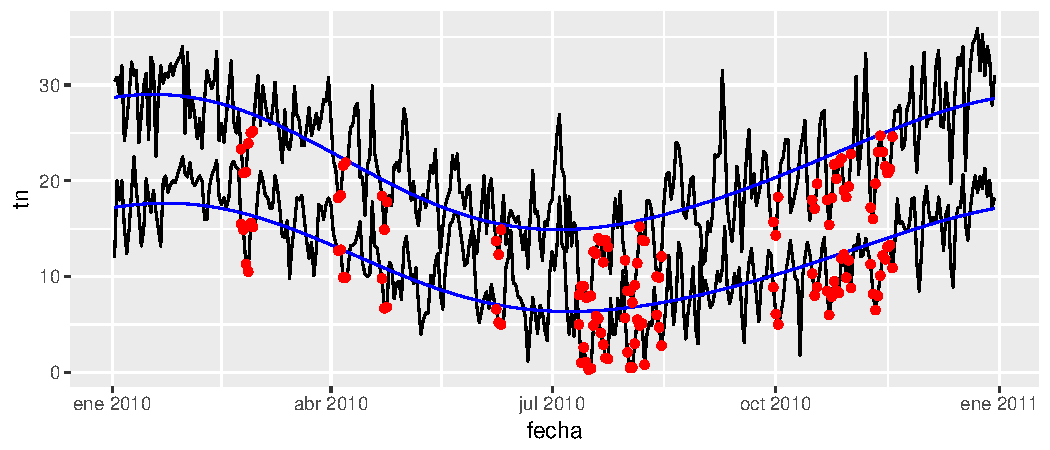
\includegraphics[width=\maxwidth]{figure/popurri-1} 

}




{\centering 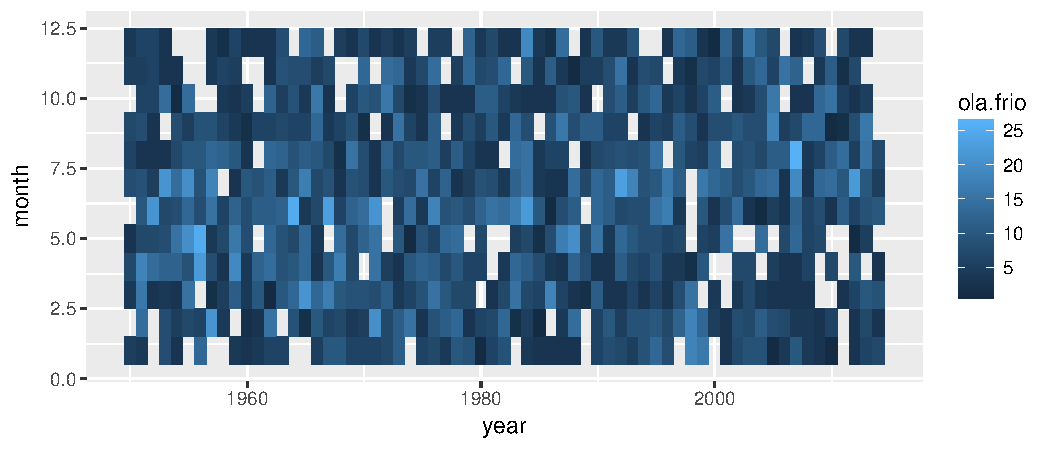
\includegraphics[width=\maxwidth]{figure/popurri-2} 

}




{\centering 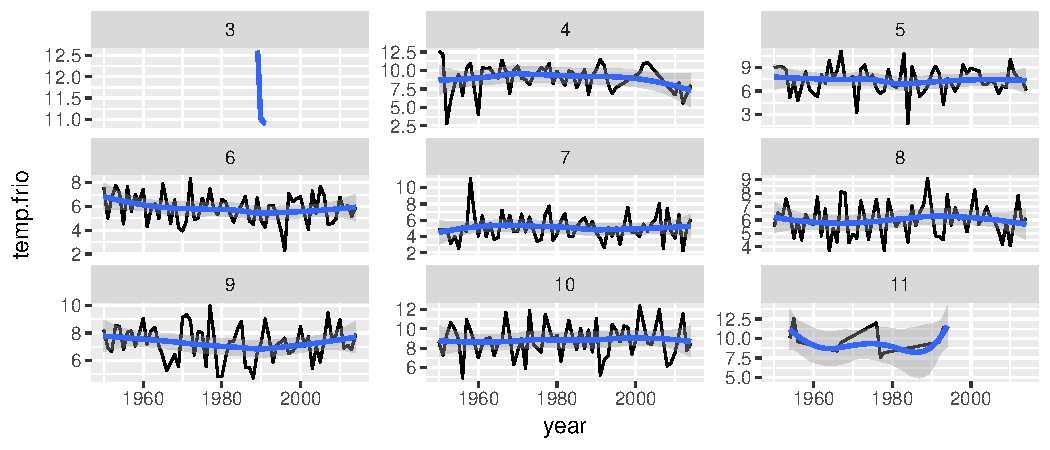
\includegraphics[width=\maxwidth]{figure/popurri-3} 

}




{\centering 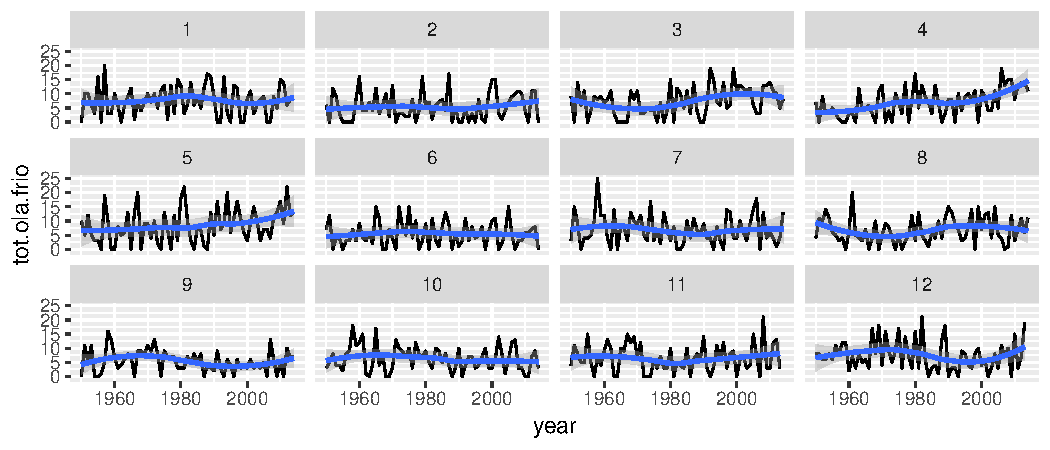
\includegraphics[width=\maxwidth]{figure/popurri-4} 

}




{\centering \includegraphics[width=\maxwidth]{figure/popurri-5} 

}




{\centering \includegraphics[width=\maxwidth]{figure/popurri-6} 

}




{\centering \includegraphics[width=\maxwidth]{figure/popurri-7} 

}



\end{knitrout}

\newpage

El objeto \verb|Tn.filter$m| tendrá la estimación.
% Lo primero es estimar la varianza observacional con la función \verb|dlmMLE|, que aproximará una estimación óptima, con un algoritmo iterativo. Para ello, primero debemos crear una función auxiliar (\verb|parMLE|), cuyo argumento sea un valor inicial propuesto para el parámetro, que retorne un objeto de la clase \verb|dlm|, en este caso de la familia de modelos trigonométricos, donde la frecuencia es 365. Le especificamos que mantenga 2 armónicos y descarte el resto:\\
% \verb|parMLE <- function(par)  dlmModTrig(s = 365,q=2, dV = par, dW = 0)|
%
% La función \verb|dlmMLE| devolverá el modelo, con el/los parámetros estimados:\\
% \verb|mod<- dlmMLE(y,parm = 16,build= parMLE)|
%
% Una vez estimado el modelo, podemos aplicar el filtro de Kalman (\verb|dlmFilter|) para obtener estimaciones de la esperanza \textit{a posteriori}:\\
% \verb|Tn.filter <- dlmFilter(y,parMLE(mod$par))|

El paquete \verb|dlm| permite trabajar con toda la familia de modelos lineales dinámicos. %La función \verb|dlmMoTrig| nos permite crear objetos \verb|dlm| de

Si el objeto \verb|y| contiene una de las series de temperaturas, el siguiente programa nos dará la estimación del modelo.

Lo primero es estimar la varianza observacional con la función \verb|dlmMLE|, que aproximará una estimación óptima, con un algoritmo iterativo. Para ello, primero debemos crear una función auxiliar (\verb|parMLE|), cuyo argumento sea un valor inicial propuesto para el parámetro, que retorne un objeto de la clase \verb|dlm|, en este caso de la familia de modelos trigonométricos, donde la frecuencia es 365. Le especificamos que mantenga 2 armónicos y descarte el resto:\\
\verb|parMLE <- function(par)  dlmModTrig(s = 365,q=2, dV = par, dW = 0)|

La función \verb|dlmMLE| devolverá el modelo, con el/los parámetros estimados:\\
\verb|mod<- dlmMLE(y,parm = 16,build= parMLE)|

Una vez estimado el modelo, podemos aplicar el filtro de Kalman (\verb|dlmFilter|) para obtener estimaciones de la esperanza \textit{a posteriori}:\\
\verb|Tn.filter <- dlmFilter(y,parMLE(mod$par))|

En la figura \ref{fig:graf6} se muestra en un período de tres años, las series de mínima y máxima y la estimación de su valor esperado mediante el filtro de Kalman.

%\section{Resultados}

% \begin{center}
% 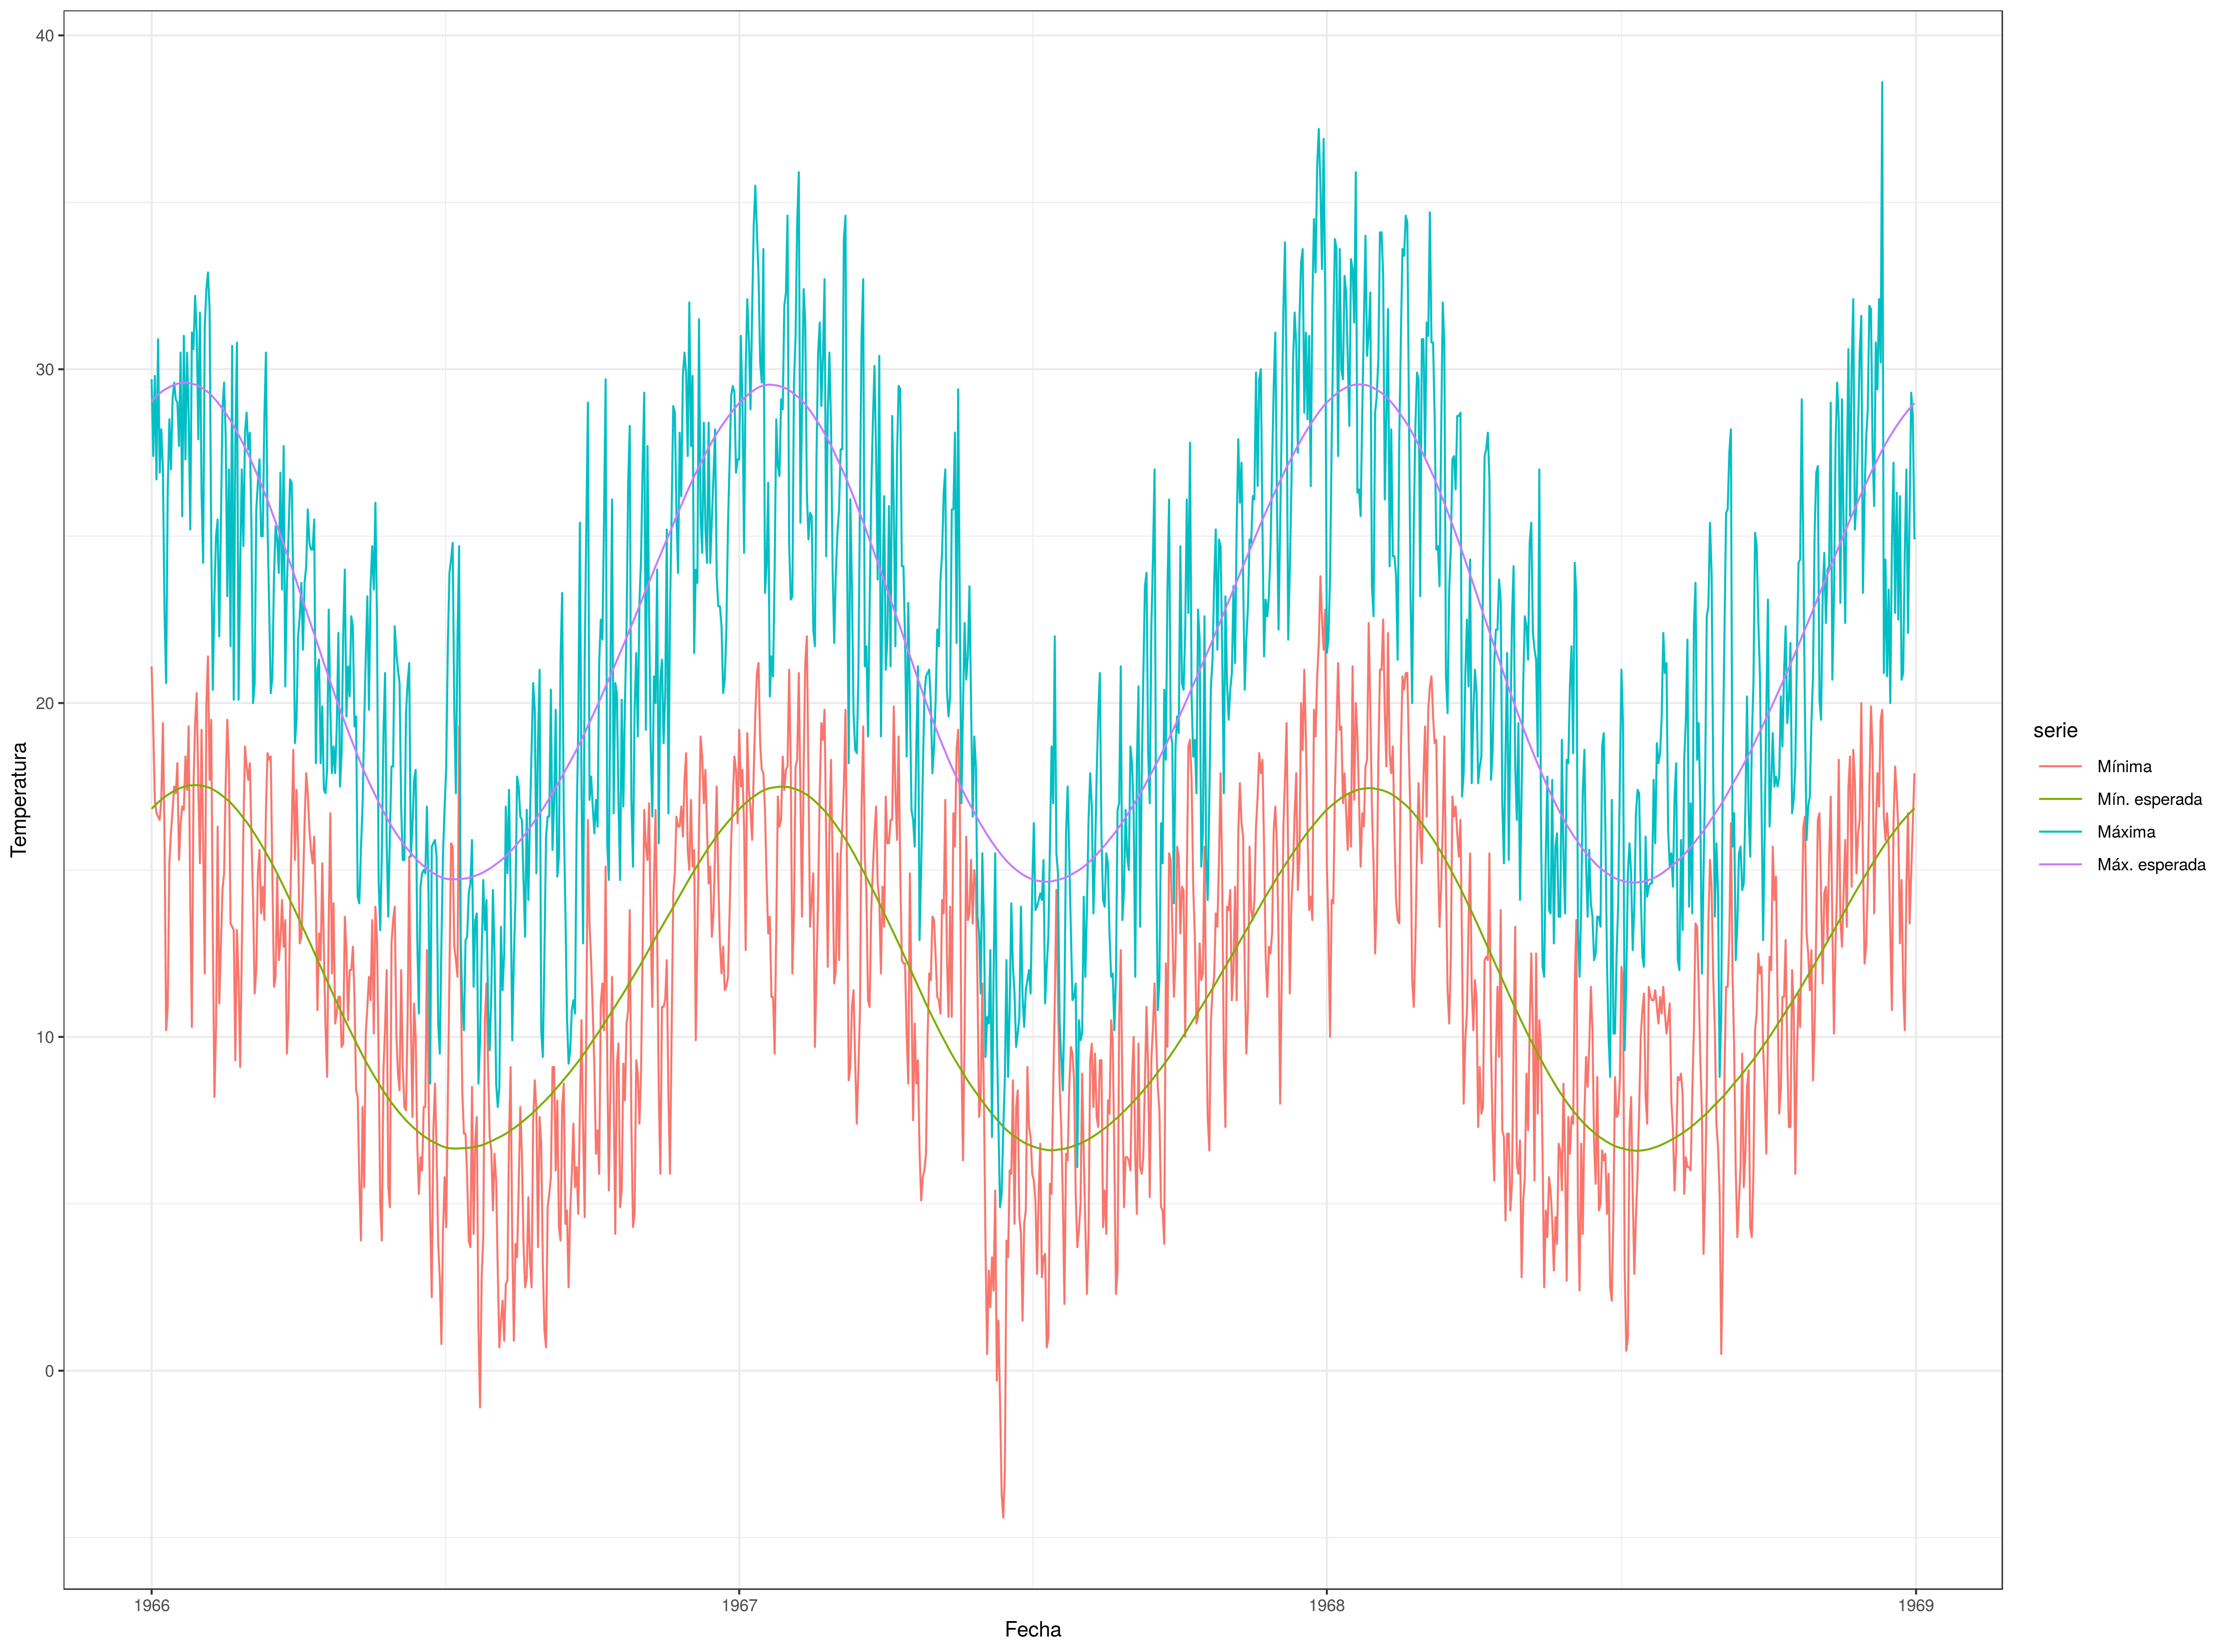
\includegraphics[width=.45\textwidth ,height=15em]{graf6.png}
% \vspace{-.75em}
% \captionof{figure}{Gráfico de mínimas y máximas del 1966 al 1969, y la estimación del valor esperado del proceso, mediante el filtro de Kalman}
% \label{fig:graf6}
% \end{center}
%
% \begin{center}
% 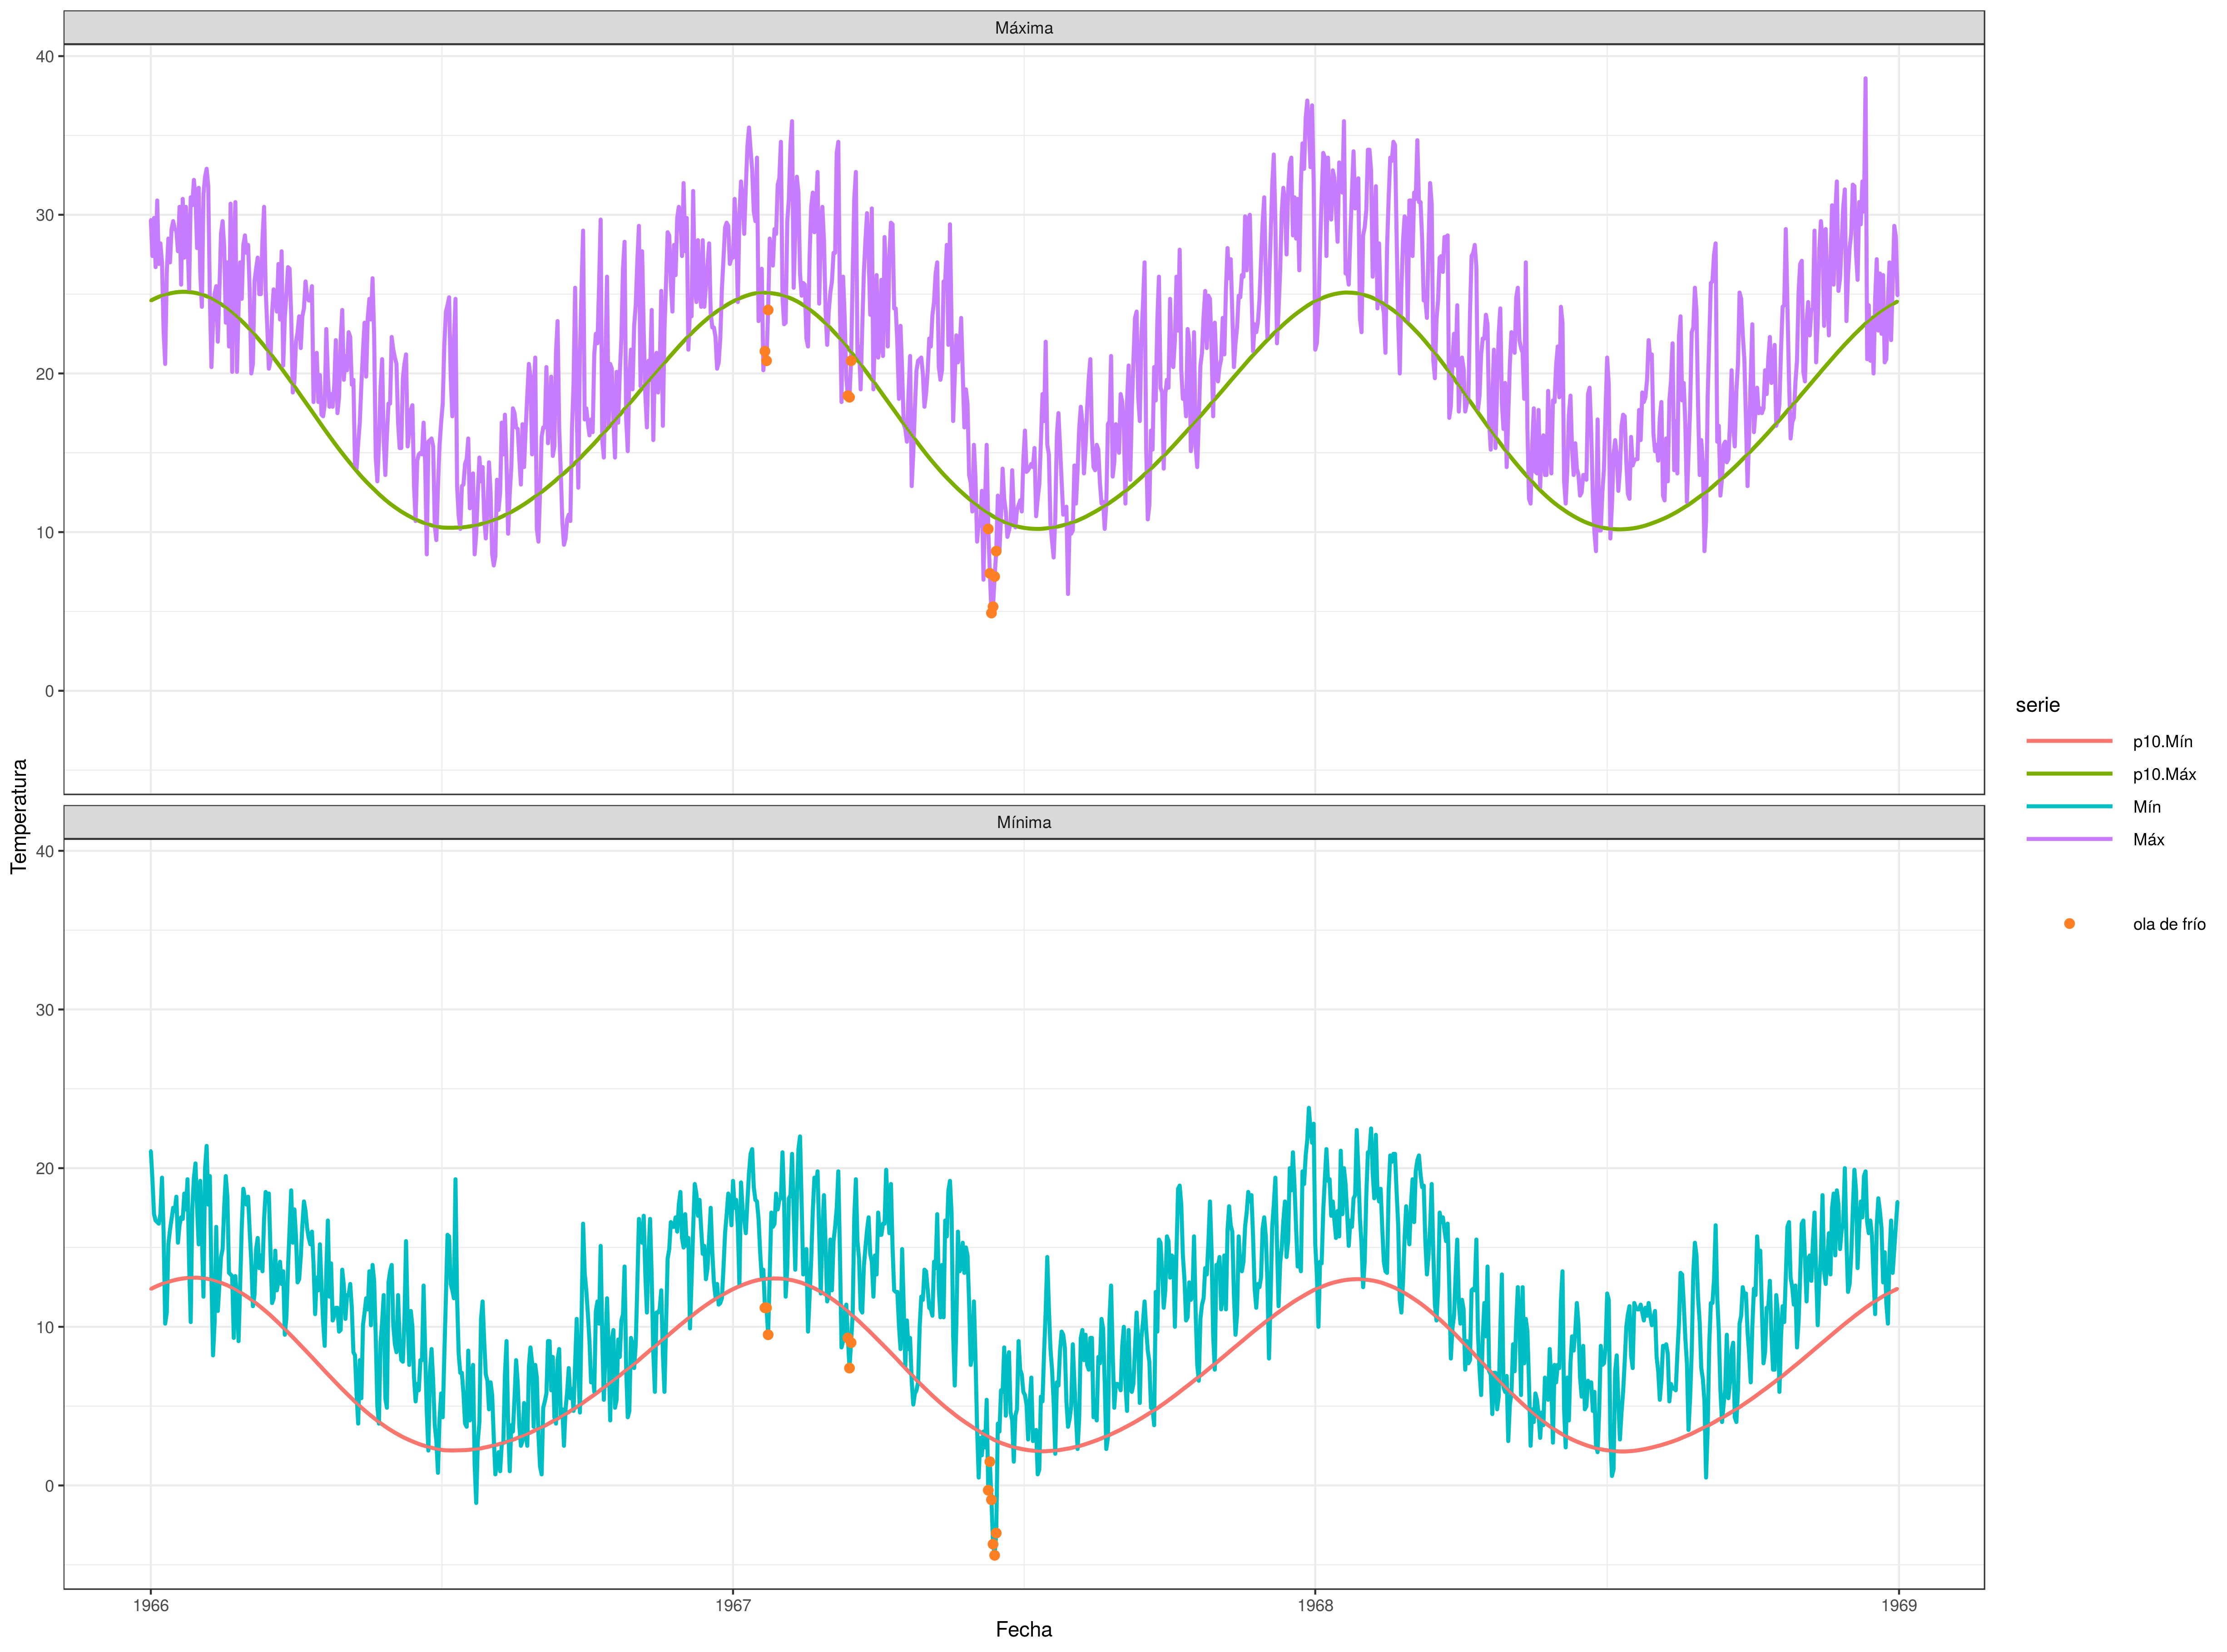
\includegraphics[width=.4\textwidth,height=21em]{graf4.png}
% \captionof{figure}{Mínimas y máximas del 1966 al 1969, percentiles 10, y olas de frío detectadas}
% \label{fig:graf4}
% \end{center}
%
% \begin{scriptsize}
% \begin{center}
% \begin{tabular}{lrrrr}
%   \hline
% Fecha & Mín & Máx & p10 mín & p10 máx \\
%   \hline
% 1967-06-09 & 5.40 & 3.14 & 15.50 & 11.25 \\
%   1967-06-10 & -0.30 & 3.08 & 10.20 & 11.19 \\
%   1967-06-11 & 1.50 & 3.03 & 7.40 & 11.12 \\
%   1967-06-12 & -0.90 & 2.97 & 4.90 & 11.06 \\
%   1967-06-13 & -3.70 & 2.92 & 5.30 & 11.00 \\
%   1967-06-14 & -4.40 & 2.86 & 7.20 & 10.94 \\
%   1967-06-15 & -3.00 & 2.81 & 8.80 & 10.88 \\
%   1967-06-16 & 3.90 & 2.77 & 12.30 & 10.83 \\
%    \hline
% \end{tabular}
% \captionof{table}{Mínimas, máximas y percentiles 10 de mínimas y máximas, en ocasión de ola de frío detectada, desde el 10 al 16 de junio de 1967, }
% \end{center}
% % \end{scriptsize}
% 

\textbf{Palabras clave}:  
\textbf{C\'ODIGOS JEL}: 
\vspace{0.5cm}
\textbf{Clasificaci\'on MSC2010}: 

\begin{center}
	\textbf{titulo in english...}
\end{center}

\begin{center}
authors ... 
\end{center}

\begin{center}
	\textbf{ABSTRACT}
\end{center}

oh boy .... 

\textbf{Key words}:  

\textbf{JEL CODES}: 

\textbf{Mathematics Subject Classification MSC2010}: 

\pagebreak
\pagestyle{fancy}
\fancyhf{}
\fancyhead[RE,LO]{titulo }
\fancyhead[LE,RO]{\thepage}
\fancyfoot[RE,RO]{autores abreviados .. }
\fancyfoot[LE,LO]{DT (17/3)-Instituto de Estadística}


\renewcommand{\refname}{Referencias Bibliográficas}

%% Bibliografica usando bibtex
% \pagebreak
% \bibliographystyle{apalike-es}
% \bibliography{biblio/poLCA}

\begin{itemize}
\item Petris, G., Petrone, S., \& Campagnoli, P. (2009). Dynamic linear models. In Dynamic Linear Models with R (pp. 31-84). Springer, New York, NY.

\item Niemi, J. (2012). STAT 615: Advanced Bayesian Methods [Beamer slides]. Retrieved from http://www.jarad.me/courses/stat615/slides/DLMs/DLMs.pdf

\end{itemize}

\pagebreak
\thispagestyle{empty}
\begin{center}

\vspace{1.5 cm}
{\Huge Instituto de Estadística} 
\noindent\rule{18cm}{0.4pt}

\vspace{0.5 cm}
\pagestyle{fancy}
{\Huge Documentos de Trabajo}\\
\thispagestyle{empty}
%\noindent\rule{18cm}{0.4pt
\includegraphics[width=0.50\textwidth]{grafi/logo_iesta.png}}
\vspace{1.5 cm}

\includegraphics[width=0.40\textwidth]{logo_iesta.png}

%\begin{center}
\thispagestyle{empty}
\vspace{4.5 cm}

\begin{flushright}
	\textbf{\large Eduardo Acevedo 1139. CP 11200
		Montevideo, Uruguay\\
		Teléfonos y fax: (598) 2410 2564 - 2418 7381\\
		Correo: ddt@iesta.edu.uy\\
		www.iesta.edu.uy\\
		Área Publicaciones\\}	
\end{flushright}

\vspace{1.5 cm}
\large\textbf{Diciembre, 2017}\\
\large\textbf{DT (17/3)}
\end{center}

\end{document}

